% EfficientNet-B4 Baseline — signal-processing paper style (monochrome, 3D tensor stacks + R-shape).
% Compile:  pdflatex fig_arch_b4_sigproc.tex
\documentclass[border=12pt]{standalone}
\usepackage{amsmath,amssymb}
\usepackage{tikz}
\usetikzlibrary{arrows.meta,calc,positioning}
\begin{document}
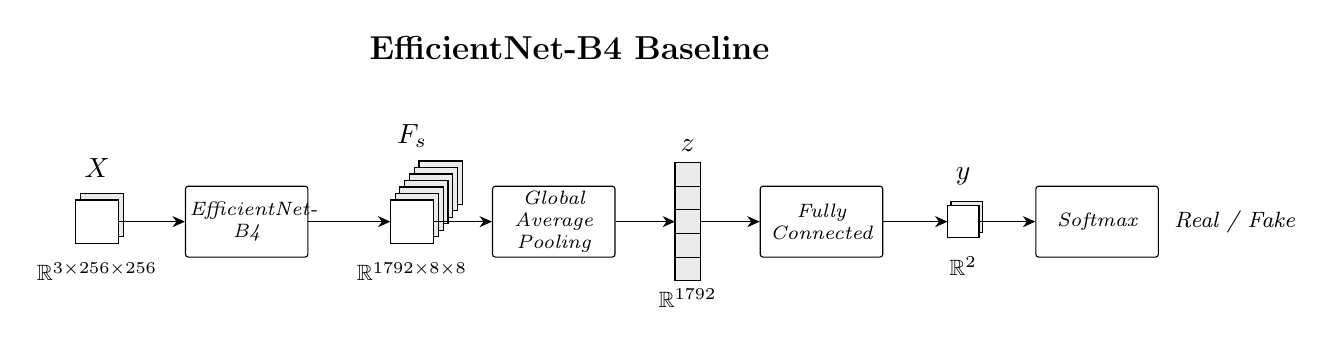
\begin{tikzpicture}[
  font=\small,
  op/.style={draw=black, thin, fill=white, rounded corners=1pt,
             text width=1.45cm, align=center, minimum height=0.9cm,
             inner sep=1.5pt, font=\scriptsize\itshape},
  arr/.style={-{Stealth[length=4.5pt,width=4pt]}, thin},
]
% ---- tensor-stack macro: #1 id #2 x #3 y #4 n #5 side #6 above #7 below ----
\newcommand{\stk}[7]{%
  \pgfmathsetmacro{\ss}{#5}\pgfmathsetmacro{\ox}{0.11*#5}\pgfmathsetmacro{\oy}{0.15*#5}%
  \foreach \i in {#4,...,1}{%
    \pgfmathtruncatemacro{\k}{\i-1}%
    \ifnum\i=1 \def\fc{white}\else \def\fc{black!8}\fi
    \pgfmathsetmacro{\xll}{#2 - \ss/2 + \k*\ox}\pgfmathsetmacro{\yll}{#3 - \ss/2 + \k*\oy}%
    \pgfmathsetmacro{\xur}{\xll + \ss}\pgfmathsetmacro{\yur}{\yll + \ss}%
    \draw[thin,fill=\fc] (\xll,\yll) rectangle (\xur,\yur);%
  }%
  \pgfmathtruncatemacro{\kn}{#4-1}%
  \pgfmathsetmacro{\ytop}{#3 + \ss/2 + \kn*\oy + 0.32}\pgfmathsetmacro{\ybot}{#3 - \ss/2 - 0.36}%
  \pgfmathsetmacro{\xw}{#2 - \ss/2}\pgfmathsetmacro{\xe}{#2 + \ss/2}\pgfmathsetmacro{\yn}{#3 + \ss/2 + \kn*\oy}%
  \node[font=\itshape] at (#2,\ytop) {#6};\node[font=\footnotesize] at (#2,\ybot) {#7};%
  \coordinate (#1-w) at (\xw,#3);\coordinate (#1-e) at (\xe,#3);\coordinate (#1-n) at (#2,\yn);%
}
\newcommand{\vbar}[5]{%
  \draw[thin,fill=black!8] (#2-0.16,#3-0.75) rectangle (#2+0.16,#3+0.75);%
  \foreach \t in {1,...,4}{\pgfmathsetmacro{\yt}{#3-0.75+\t*0.3}\draw[thin] (#2-0.16,\yt)--(#2+0.16,\yt);}%
  \node[font=\itshape] at (#2,#3+0.97) {#4};\node[font=\footnotesize] at (#2,#3-0.97) {#5};%
  \coordinate (#1-w) at (#2-0.16,#3);\coordinate (#1-e) at (#2+0.16,#3);%
}

% ---- stacks ----
\stk{X}{0}{0}{2}{0.55}{$X$}{$\mathbb{R}^{3\times256\times256}$}
\stk{Fs}{4.0}{0}{7}{0.55}{$F_s$}{$\mathbb{R}^{1792\times8\times8}$}
\vbar{z}{7.5}{0}{$z$}{$\mathbb{R}^{1792}$}
\stk{Yy}{11.0}{0}{2}{0.40}{$y$}{$\mathbb{R}^{2}$}

% ---- operations (full readable names) ----
\node[op] (B4)  at (1.9,0)  {EfficientNet-B4};
\node[op] (GAP) at (5.8,0)  {Global\\Average Pooling};
\node[op] (FC)  at (9.2,0)  {Fully\\Connected};
\node[op] (SM)  at (12.7,0) {Softmax};

% ---- edges ----
\draw[arr] (X-e)  -- (B4.west);
\draw[arr] (B4.east) -- (Fs-w);
\draw[arr] (Fs-e) -- (GAP.west);
\draw[arr] (GAP.east) -- (z-w);
\draw[arr] (z-e) -- (FC.west);
\draw[arr] (FC.east) -- (Yy-w);
\draw[arr] (Yy-e) -- (SM.west);
\node[font=\footnotesize,right=2pt of SM] {\itshape Real / Fake};

% ---- title ----
\node[font=\bfseries\large] at (6.0,2.2) {EfficientNet-B4 Baseline};
\end{tikzpicture}
\end{document}
